\documentclass[resume]{subfiles}


\begin{document}
\section{Signaux et systèmes en temps discret}
$$x(n)=x_\text{continu}(nT_s)$$
Avec $T_s$ la période d'échantillonnage
\paragraph{Impulsion unité}
$$\delta(n)=\begin{cases}1 & n=0\\0 & n\neq 0\end{cases}$$
$$x(n)=\sum_{k=-\infty}^{\infty}x(k)\delta(n-k)$$
\paragraph{Saut unité}
$$u(n)=\begin{cases}1 & n \geq 0 \\0 & n < 0\end{cases}$$
\paragraph{Durée finie} : échantillons égaux à 0 en dehors d'un intervalle donné
\paragraph{Durée infinie} : saut unité, oscillation, etc...
\paragraph{Séquence à droite} : $0$ pour $n<n_0$
\paragraph{Séquence à gauche} : $0$ pour $n>n_0$
\paragraph{Représentation exponentielle d'un signal périodique}
$$e^{\sigma n + jn\omega_0}=e^{\sigma n}\left(\cos(n\omega_0)+j\sin(n\omega_0)\right)$$
Pas d'amortissement si $\sigma=0$
\subsection{Propriétés des systèmes}
Lorsqu'on passe un signal $x$ dans un système $T$ on obtient une sortie $y$
$$y(n)=T\left[x(n)\right]$$
$$\boxed{y(n)=\sum_{k=0}^{q}\bcolor{b}(k)x(n-k)-\sum_{k=1}^{p}\acolor{a}(k)y(n-k)}$$
$$\begin{cases}
\text{IIR} & a(k) \neq 0\quad \forall k\in 1,...,p\\
\text{FIR} & a(k) = 0\quad \forall k\in 1,...,p
\end{cases}$$
$$p>q\longrightarrow\text{ causal}$$
$p$ est l'ordre du système
\paragraph{Linéarité}
$$T\left[ax_1(n)+bx_2(n)\right]=aT\left[x_1(n)\right]+bT\left[x_2(n)\right]$$
\paragraph{Invariance temporelle (ou shift)}
$$y(n-n_0)=T\left[x(n-n_0)\right]$$
\paragraph{Causalité}
$y(n)$ dépend uniquement de $y(n-k)$ et $x(n)$
\paragraph{Stabilité}
BIBO : borné en entrée et borné en sortie. Vérifié si
$$\sum_{n=-\infty}^{\infty}\abs{h(n)} < \infty$$
\paragraph{Inversibilité}
Si on peut déterminer $x(n)$ à partir de $y(n)$
$$x_1(n)\neq x_2(n)\longrightarrow y_1(n)\neq y_2(n)$$
\subsection{Convolution}
\subsubsection{Propriétés}
\paragraph{Linéarité}
$$x(n)*(\alpha y(n)+\beta w(n))=\alpha x(n)*y(n) + \beta x(n)*w(n)$$
\paragraph{Invariance temporelle}
$$w(n)=x(n)*y(n)\Longleftrightarrow x(n)*y(n-k)=w(n-k)$$
\paragraph{Commutativité}
$$x(n)*y(n)=y(n)*x(n)$$
\paragraph{Associativité}
$$\Big(x(n)*h(n)\Big)*w(n)=x(n)*\Big(h(n)*w(n)\Big)$$
\paragraph{Multiplication par une impulsion unité}
$$h(n)*d(n)=h(n)$$
\subsection{DTFT}
$$\boxed{X\left(e^{j\omega}\right)=\sum_{n=-\infty}^{n=+\infty}x(n)e^{-jn\omega}}$$
Cas spéciaux :
$$x(n)=e^{jn\omega_0}\longrightarrow X\left(e^{j\omega}\right)=2\pi u(\omega-\omega_0)\quad \abs{\omega}<\pi$$
$$x(n)=u(n)\longrightarrow X\left(e^{j\omega}\right)=\frac{1}{1-e^{-j\omega}}+\pi u(\omega)\quad \abs{\omega}<\pi$$
Impulsion unité :
$$H(e^{j\omega})=\sum_{n=-\infty}^{+\infty}h(n)e^{-jn\omega}$$
$H$ décrit la réponse fréquentielle du système
\subsubsection{Propriétés}
\paragraph{Périodicité} $X(e^{j\omega})$ est périodique en $2\pi$
\paragraph{Signal réel} si $x(n)$ réel alors
$$x(e^{j\omega})=X^\ast\left(e^{-j\omega}\right)$$
\paragraph{Décomposition amplitude-phase}
$$X(e^{j\omega})=\abs{X(e^{j\omega})}e^{j\Phi_x(\omega)}$$
Pour un signal réel $\abs{X(e^{j\omega}}$ est paire et $\Phi$ impaire
\subsubsection{Opérations}
\paragraph{Convolution}
$$y(n)=x(n)*h(n)\Longleftrightarrow Y(e^{j\omega})=X(e^{j\omega})\cdot H(e^{j\omega})$$
\paragraph{Modulation}
$$y(n)=x(n)\cdot h(n)\Longleftrightarrow Y(e^{j\omega})=X(e^{j\omega})*H(e^{j\omega})$$
\subsection{Transformée en $z$}
$$X(z)=\sum_{n=-\infty}^{+\infty}x(n)z^{n}\qquad z=re^{j\omega}$$
\begin{figure}[H]
\centering
\includegraphics[width=0.9\columnwidth,page=3]{drwg_2.pdf}
\end{figure}
Si une fréquence tombe pile sur un zéro (sur le cercle unité) alors elle sera complètement annulée. Un pôle proche du cercle unité va augmenter les fréquences proches de ce pôle.
\subsubsection{Propriétés}
\paragraph{Linéarité}
$$Z\lbrace \alpha x(n)+\beta y(n)\rbrace=\alpha X(z)+\beta Y(z)$$
\paragraph{Décalage temporel}
$$Z\lbrace x(n-N)\rbrace=z^{-N}X(z)$$
\begin{table}[H]
\begin{tabular}{lcc}
 & $x(n)$ & $X(z)$\\\hline
Délai & $x(n-n_0)$ & $z^{-n_0}X(z)$\\
Multiplication par $\alpha^{n}$ & $a^{n}x(n)$ & $X(z/\alpha)$\\
Conjugué & $x^\ast(n)$ & $X^\ast(z^\ast)$\\
Inversion de temps & $x(-n)$ & $X(z^{-1})$\\
Convolution & $x(n)*w(n)$ & $X(z)W(z)$\\
Multiplication par $n$ & $nx(n)$ & $-z\frac{d}{dz}X(z)$
\end{tabular}
\caption{Opérations}
\end{table}
$$Z\lbrace\delta(n)\rbrace=1$$
\subsection{Équation aux différences}
$$\underset{\text{degré relatif}}{d}=\underset{\deg(\text{denominateur})}{n}-\underset{\deg(\text{numérateur})}{m}$$
\begin{small}
$$G(z)=\frac{Y(z)}{X(z)}$$
$$G(z)=\frac{\bcolor{b_0}z^{-d}+\bcolor{b_1}z^{-d-1}+\bcolor{b_2}z^{-d-2}+\cdots+\bcolor{b_m}z^{-d-m}}{\textcolor{Gray}{a_0}+\acolor{a_1}z^{-1}+\acolor{a_2}z^{-2}+\cdots+\acolor{a_n}z^{-n}}$$
\end{small}
$a\longrightarrow \text{ poles}$, $b\longrightarrow\text{ zéros}$
$$\abs{a_i}<1\longrightarrow\text{ stable}\quad \forall i\in [1,n]$$
\end{document}